% Created 2023-01-20 Пт 00:40
% Intended LaTeX compiler: pdflatex
\documentclass[PI, VKR]{HSEUniversity}
         \usepackage{array,tabularx,tabulary,booktabs,longtable,multirow}
         \Year{\the\year{}}
         \supervisor{к.т.н., доцент кафедры информационных технологий в бизнесе НИУ ВШЭ-Пермь}{А. В. Бузмаков}
                  \Abstract{В данной работе проведен анализ этичности разных компаний.

В первой главе находится описание используемых алгоримов.

Во второй главе представлено проектирование системы.

В третьей главе представлена реализация системы.

В четвертой главе представлено тестирование работы системы.

Количество страниц - N, количество иллюстраций - N, количетсво таблиц - N.}


\usepackage[utf8]{inputenc}
\usepackage[T1]{fontenc}
\usepackage{graphicx}
\usepackage{longtable}
\usepackage{wrapfig}
\usepackage{rotating}
\usepackage[normalem]{ulem}
\usepackage{amsmath}
\usepackage{amssymb}
\usepackage{capt-of}
\usepackage{hyperref}
\author{Соломатин Роман Игоревич}
\date{\today}
\title{Разработка сайта для автоматического сбора, анализа и визуализации информации по этичности компаний}
\hypersetup{
 pdfauthor={Соломатин Роман Игоревич},
 pdftitle={Разработка сайта для автоматического сбора, анализа и визуализации информации по этичности компаний},
 pdfkeywords={},
 pdfsubject={},
 pdfcreator={Emacs 28.2 (Org mode 9.6)},
 pdflang={Ru}}
\usepackage{biblatex}
\addbibresource{/home/samoed/Desktop/ESGanalysis/docs/library.bib}
\addbibresource{~/Desktop/notes/org/bibliography.bib}
\begin{document}

\maketitle

\chapter*{Введение}
\label{sec:org79e69d8}
Этичность компаний уже давно вызывает озабоченность, особенно в отношении их поведения в спорных ситуациях и предоставления услуг, ориентированных на клиента. В последние годы все большее внимание уделяется оценке этичности компаний\autocites[]{mure_esg_2021}[][]{miralles-quiros_esg_2019}[][]{climent_ethical_2018}, особенно в банковском секторе и через призму экологических, социальных и управленческих факторов (ESG). Необходимость в таких оценках становится все более острой по мере того, как общество продолжает бороться с последствиями неправомерных действий корпораций и более широким воздействием корпоративной деятельности на общество и окружающую среду.

В настоящее время существует несколько сервисов, которые призваны оценивать этику компании, но эти оценки часто основаны на судебных делах и других официальных отчетах, а не на отзывах клиентов. Это привело к ситуации, когда отдельные лица должны проводить свои собственные исследования, чтобы определить насколько этична компания. Это часто включает в себя просмотр отзывов с различных веб-сайтов, что может занять много времени и не всегда может дать исчерпывающую или точную картину.

Для решения этой проблемы будет реализована система, которая собирала бы и анализировала отзывы потребителей с различных веб-сайтов, чтобы дать более полную и точную оценку этической практики компании. Такая система может быть разработана для автоматического сбора и анализа отзывов потребителей из различных источников, включая социальные сети и сайты отзывов. Затем собранные данные могут быть проанализированы с помощью различных методов, таких как обработка естественного языка и машинное обучение, для выявления закономерностей и тенденций, связанных с этической практикой компании. Полученный анализ может быть использован для разработки более надежной и достоверной системы оценки этичности компаний.

Объект исследования – деятельность компаний.

Предмет исследования – программные средства для оценки этичности деятельности компаний.

Цель работы – создание системы для оценки этичности компаний.

Исходя из поставленной цели, необходимо:

\begin{enumerate}
\item Провести анализ предметной области
\item Провести анализ системы
\item Реализовать систему
\item Провести тестирование системы
\end{enumerate}

Этап анализа должен:
\begin{enumerate}
\item Анализ предметной области
\item Анализ существующих алгоритмов
\end{enumerate}

Этап проектирования должен включать:
\begin{enumerate}
\item Проектирование серверной части
\item Проектирование модели для определения этичности
\item Проектирование клиентской части приложения
\end{enumerate}

Этап реализации должен включать:
\begin{enumerate}
\item Описание сбора данных
\item Реализации модели
\item Реализации серверной части
\item Реализации клиентской части
\end{enumerate}

Этап тестирования должен включать:
\begin{enumerate}
\item Тестирование модели
\item Тестирование серверной части
\item Тестирование клиентской части
\end{enumerate}
\chapter{Анализ предметной области}
\label{sec:orgf0e2f86}
\section{BERT}
\label{sec:org3a1a545}
BERT \autocite{devlin2018bert} (Bidirectional Encoder Representations from Transformers) -- это нейросетевая языковая модель, которая показала высокую эффективность для задач обработки естественного языка, таких как классификация текстов, ответы на вопросы и распознавание именованных сущностей. Она основана на архитектуре трансформаторов, представленной в статье "Attention is All You Need" \autocite{NIPS2017_3f5ee243}, которая использует механизмы самовнимания для обработки входных последовательностей параллельно, а не последовательно, как в традиционных архитектурах рекуррентных нейронных сетей.

В отличие от простых алогитмов машинного обучения, таких как, TF-IDF \autocite{jones1972statistical}, мешка слов\autocite{doi:10.1080/00437956.1954.11659520} и word2vec \autocite{mikolov2013efficient} последовательности слов и предложений кодируются вектором (эмбеддингом) фиксированной длины. Это позволяет эффективно анализировать текст с пониманием контекста, что поможет при анализе отзывов.
Одной из основных причин превосходной производительности BERT является его способность работать с двунаправленным контекстом. В отличие от ELMO \autocite{elmo} и GPT\autocite{radford2019language}, которые являются однонаправленными моделями, BERT обучен учитывать контекст как слева, так и справа от слова, что приводит к более точному представлению значения слов в предложении.

На вход модели подается предложение или пара предложений. Затем разделяется на отдельные слова (токены).  Потом в начало последовательности вставляется специальный токен \texttt{[CLS]}, обозначающий начало предложения или начало последовательности предложений. Пары предложений группируются в одну последовательность и разделяются с помощью специального токена \texttt{[SEP]}. Потом все токены превращаются в эмбеддинги \ref{fig:inputemebeddings} по механизму внимания \autocite{NIPS2017_3f5ee243}.

\begin{figure}[h]
\centering
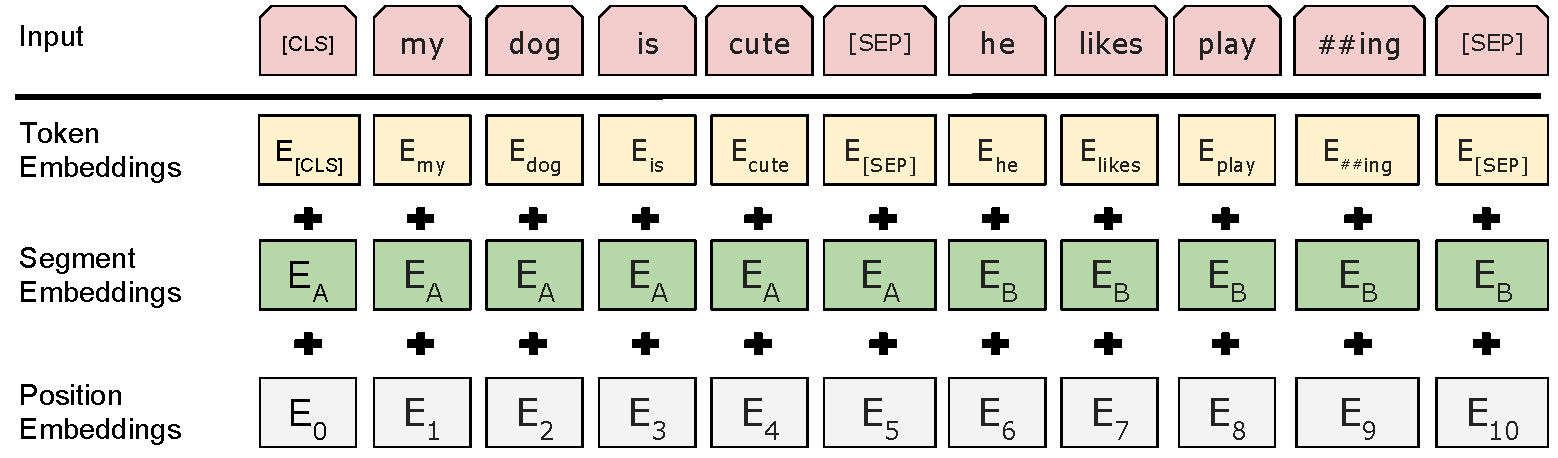
\includegraphics[width=.9\linewidth]{img/Input_Emebeddings.pdf}
\caption{\label{fig:inputemebeddings}Пример ввода текста в модель}
\end{figure}

При обучении модель выполняет на 2 задания:
\begin{enumerate}
\item Предсказание слова в предложении

Поскольку стандартные языковые модели или смотрят текст слева направо, или справа налево \ref{fig:BERT_comparisons}, как ELMo \autocite{elmo} и GPT \autocite{radford2019language}, они работают с контекстом хуже, чем данная модель. Так как BERT двунаправленный, у каждого слова можно посмотреть его контекст, что позволит предсказать замаскированное слово.

\begin{figure}[h]
\centering
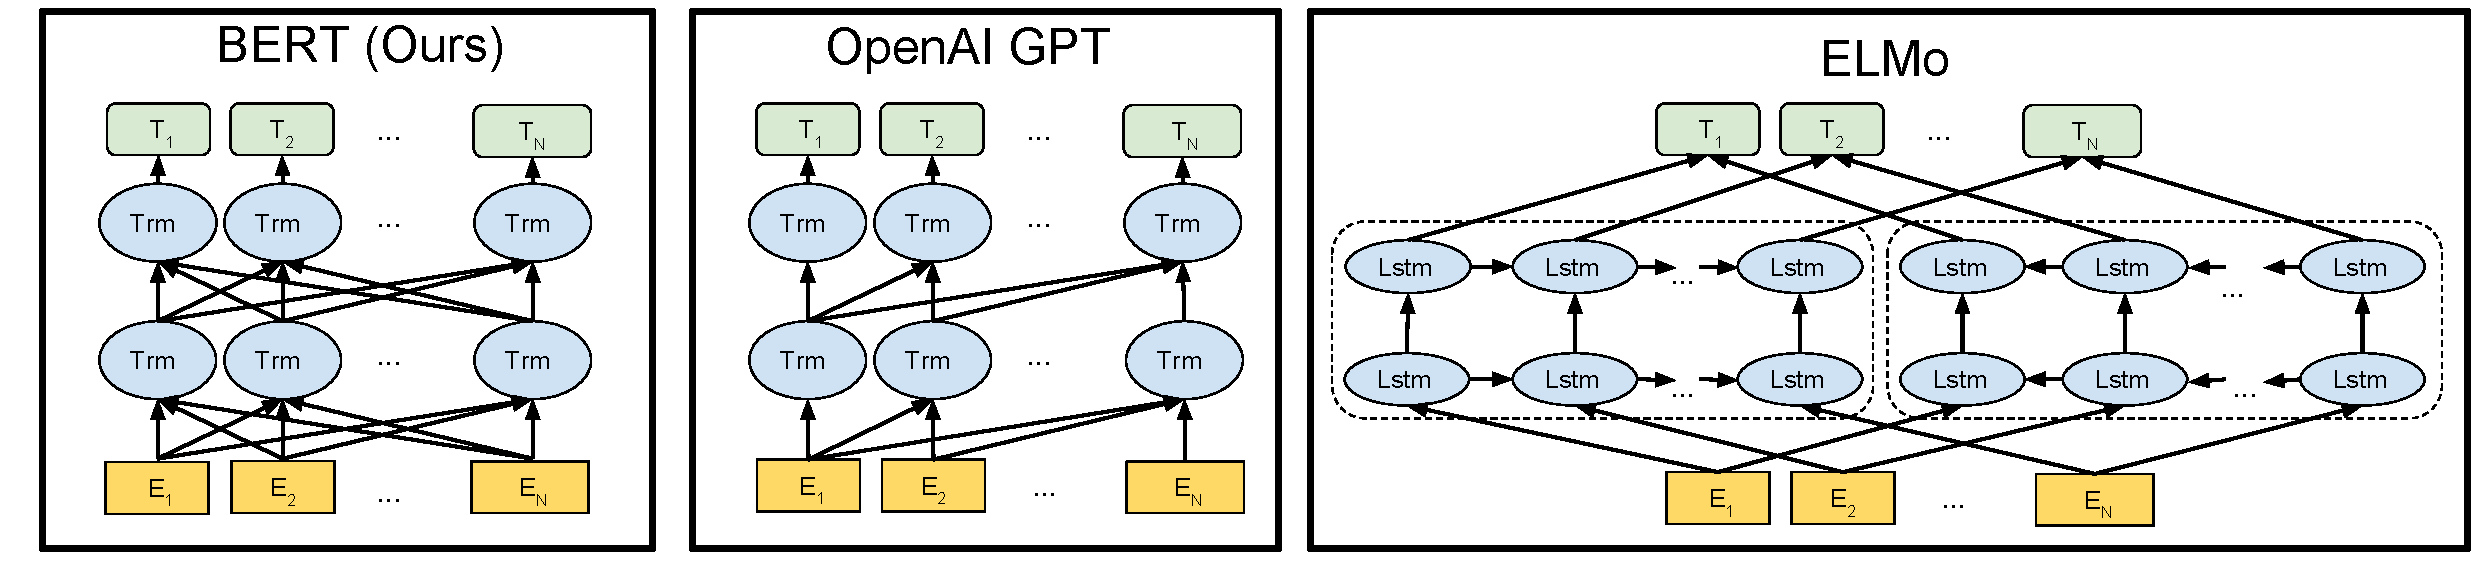
\includegraphics[width=.9\linewidth]{img/BERT_comparisons.pdf}
\caption{\label{fig:BERT_comparisons}Сравнение принципов работы BERT, ELMo, GPT}
\end{figure}

Это задание обучается следующим образом -- 15\% случайных слов заменяются в каждом предложении на специальный токен \texttt{[MASK]}, а затем предсказываются, учитывая окружающий контекст. Однако иногда слова заменяются не на специальные токены, в 10\% заменяются на случайный токен и еще в 10\% заменяются на случайное слово. Этот процесс обучения позволяет модели изучить связи между словами в предложении и представить каждое слово в высокоразмерном векторном пространстве, называемом вкраплением. Эти вкрапления отражают смысл слов в предложении и могут быть использованы для представления предложения в целом.

\item Предсказание следующего предложения

Для того чтобы обучить модель, которая понимает отношения предложений, она предсказывает, идут ли предложения друг за другом. Для этого с 50\% вероятностью выбирают предложения, которые находятся рядом и наоборот. Пример ввода пары предложений в модель \ref{fig:bert_pretraining}.

\begin{figure}[!hbp]
\centering
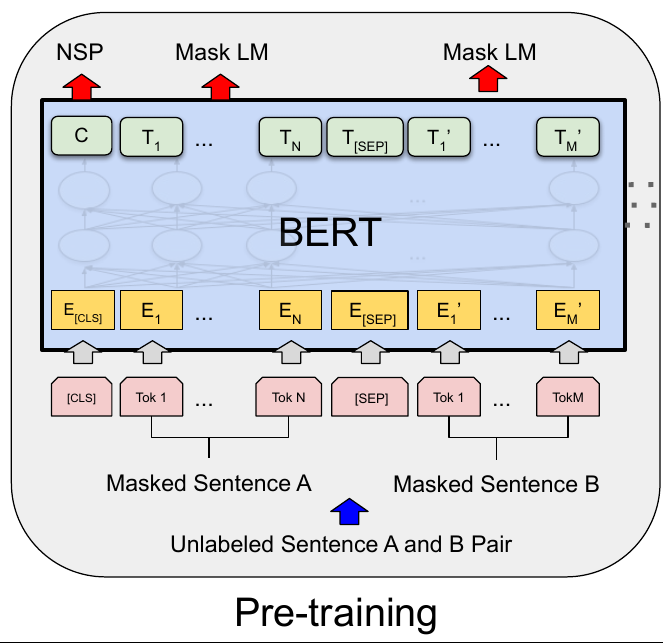
\includegraphics[width=0.6\textwidth]{img/bert_pretrainin.png}
\caption{\label{fig:bert_pretraining}Схемам работы BERT}
\end{figure}
\end{enumerate}

BERT можно использовать для получения оценки тональности отзывов о компаниях, для этого можно немного модифицировать. Он может быть обучен предсказывать, является ли отзыв положительным, отрицательным или нейтральным. После обучения модель можно будет использовать для прогнозирования тональности новых отзывов, обеспечивая надежный и эффективный способ оценки тональности отзывов о компаниях.
\section{Sentense BERT}
\label{sec:orgf91b8f1}
Sentense BERT \autocite{reimers-2019-sentence-bert} -- это модификация предобученных моделей BERT, которая использует модель BERT и подает на вход 2 предложения, затем усреднят их выходы, а после с помощью функции ошибки выдаёт результат. Схема работы модели \ref{fig:sbert}.
\begin{figure}[hbp]
\centering
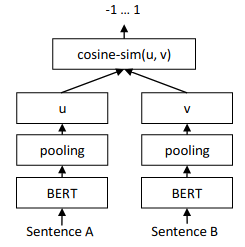
\includegraphics[width=0.4\textwidth]{img/sbert.png}
\caption{\label{fig:sbert}Схема работы SBERT}
\end{figure}
Основное преимущество данной модели над классическим BERT: эмбеддинги предложений можно сравнивать друг с другом независимо и без необходимости пересчитывать их каждый раз. Например, если для поиска похожих предложений из 10000 для обычного BERT потребуется 50 миллионов вычислений различных пар предложений, и это займёт 50 часов, то Sentense BERT рассчитает эмбеддинг каждого предложения отдельно и потом их сравнит, и это займёт примерно 5 секунд.
\section{CLIP}
\label{sec:orga2d73b5}
CLIP (Contrastive Language–Image Pre-training)\autocite{radford2021learning} -- это нейронная сеть, обученная на множестве пар (изображение, текст) и способная изучать широкий спектр визуальных и лингвистических концепций, предсказывая текст, соответствующий заданному изображению.

Модель использует Visual Transformer (ViZ) \autocite{dosovitskiy2020image} для обучения представлениям изображений. ViZ обучен понимать и генерировать изображения, а трансформер\autocite{NIPS2017_3f5ee243} обучен понимать и генерировать текст. Сочетание этих двух архитектур позволяет модели CLIP одновременно изучать визуальные и лингвистические концепции.

Одним из ключевых преимуществ CLIP является его способность обучать эмбеддинги, которые не являются специфическими для конкретной задачи или области. Кроме того, CLIP можно точно настроить на наборе данных, специфичном для конкретной задачи, чтобы улучшить производительность на конкретных задачах. Этот метод позволяет соединить пространства двух разных источников информации. Например, эта модель может быть адаптирована для соединения предложений из разных областей.
\chapter{Проектирование системы}
\label{sec:org304a460}
\section{Проектирование базы данных}
\label{sec:orgc2334b2}

\section{Проектирование архитектуры системы}
\label{sec:orgb4f09d7}
\subsection{Проектирование серверной части}
\label{sec:orgca80a85}
\subsection{Проектирование клиентской части}
\label{sec:orga7a0768}

\chapter{Реализация системы}
\label{sec:org4a0e83b}
\section{Реализация серверной части}
\label{sec:orgfc55500}
\subsection{Реализация API}
\label{sec:orgcb3e6dd}
\subsection{Реализация парсера banki.ru}
\label{sec:org304ddbd}
\subsection{Реализация парсера sravni.ru}
\label{sec:orgd0c4eba}
\subsection{Реализация модуля обработки текста}
\label{sec:orgc50799a}
\section{Реализация клиентской части}
\label{sec:orgd52c18a}
\chapter{Тестирование системы}
\label{sec:orgdcfd001}
\chapter*{Заключение}
\label{sec:org639b440}
%\nocite{*}
\putbibliography
\appendix
\end{document}
